%Asynchronous AGREE AADL Execution and Scheduling Model
%A system consists of a set of threads, a schedule, and a set of AGREE contracts.
{\bf signal.}
A signal $x$ is a sequence of values $(x_1, x_2, ...)$ of a certain data type. That is, $x = N \mapsto T$, where $x_i$ is of type $T$ for all $i \in N$. The data type can be either a primitive data type (e.g. real, bool, int, and enumeration types) or a composite data type (e.g. record types). Assume the data type of signal $x$ and $y$ is $T_x$ and $T_y$, respectively, $x = y$ means that $T_x=T_y$ and $x_i = y_i$ for all $i \in N$. 

{\bf thread.}
We model the ports of an AADL thread as signals. In particular, an event port is modelled as a sequence of Boolean values. The value \emph{true} or \emph{false} indicates an event is \emph{present} or \emph{absent} at the port, respectively. An event data port is modelled as a pair of signals, one representing the data stream, and the other representing the associated event stream. To simplify the notation, we use the port name $p$ to denote its associated \emph{data signal}, and $event(p)$ to denote its associated \emph{event signal}. The ports of a thread are divided into two finite disctinct sets: input ports ($I$) and output ports ($O$). Correspondingly, the associated signals are divided int to input signals and output signals. We model the \emph{state} of a thread with a finite set $S$ of signals. %The next state function is $T: S x I \mapsto S'$. The output function is $T: S x I \mapsto S$. Then, a thread is %A thread is modelled as a collection of input signals and output signals. A thread could be aossciated with /emph{local} states, which are not accessible outside the scope of the thread. They are modelled as signals, noted as set S . 

{\bf composition.}
An AADL \emph{connection} between an input port $i$ of one thread and an output port $o$ of another thread enforces the equality of their associated signals. For data ports, this means $i = o$. For event data prots, this means $i = o$ and $event(i) = event(o)$. %For simplicity, we define $e(p) = false^*$ if $p$ is a data port.

{\bf virtual events.}
We introduce two virtual input event ports: \emph{dispatch} ($d$) and \emph{complete} ($c$) for each thread.  The \emph{Dispatch} and \emph{Complete} event models, respectively, the start and end of the time slot that a scheduler allocated to a thread to run. 
%{\bf thread execution.}
When its \emph{dispatch} event $d$ is present, a thread samples the input values and starts execution. This is the time when the associated AGREE \emph{assumptions} $A$ should hold. That is,
$$event(d)_i \Rightarrow a_i, \forall i\in N, \forall a \in A $$

When its \emph{complete} event $c$ is present, a thread updates its ouput signal $o$ value, otherwise it holds its previous value. That is, 
$$\lnot event(c)_i \Rightarrow ((o_i = o_{i-1}) \land (event(o)_i = event(o)_{i-1}), \forall i \in N, \forall o \in O$$
The definition combined with the pervious definition of \emph{connection} models the asynchronous communication. It could be viewed as a buffer (or queue) of size one. It overwrites when overflow occurs. Note that, unlike synchronous dataflow models, the data (\emph{token}) is not disgarded after \emph{consumption}. That is, reading is non-destroying. In case of \emph{upsampling}, the consumer samples the same value repeatedly. It could also be viewed as a shared variable, which has one writer and possibly multiple readers. Since under our MoC, at most one thread is active at a time, there is no ambiguity on the order of read/write actions.

A thread updates its the state signal $s$ similarly. That is,
$$\lnot event(c)_i \Rightarrow ((s_i = s_{i-1}) \land (event(s)_i = event(s)_{i-1}), \forall i \in N, \forall s \in S$$
This is the time where the associated AGREE \emph{gurarantees} $P$ should hold. That is,
$$event(c)_i \Rightarrow p_i, \forall i\in N, \forall p \in P $$
Here we assume a thread always completes its execution within the assigned time slot. Thus, there is no pre-emption. 

%We denote the initial value of a signal as $x_0$. For an event port $p$, $e(p_0) = false$. The output write action is also non-blocking. In other words, a thread will not halt its execution due to waiting for an previous output data to be \emph{consumed}. It overwrites.

{\bf schedule.}
A schedule $\sigma$ defines when a thread out of a set of threads $P$ is activated. That is,  
$$\sigma = \{(d(p), c(p)), \forall p \in P  \}$$ 
We assume schedules are static, periodic, and valid. A schedule is called valid if in each period or \emph{cycle}, there is no other scheduling event between the \emph{dispatch} and \emph{complete} of the same thread, and the \emph{dispatch} event occurs before the matching \emph{complete} event. 

All signals by definition are associated with the same logic clock, indicated by its index. The \emph{tick} models the basic time unit where the system is analyzed. This could be the basic time unit used in a schedule, or the greatest common divisor. For example, given a schedule with a period of 10 ms, starting with thread A 4 ms, idle 2 ms, thread B 2 ms, idle 2 ms, then a model of the schedule could be $\sigma = \{d(A)=(1,0,0,0,0)^*, c(A) = (0,0,1,0,0)^*, d(B) = (0,0,0,1,0)^*, c(B) = (0,0,0,0,1)^*\}$, where each \emph{tick} models 2 ms. We introduce a circular counter to model a schedule in AGREE. The counter updates at each tick. The maximum count models the period of the schedule. 
%		-- Counter starts with init + incr, reset to init
\begin{verbatim}
		node Counter (init: int, incr: int, reset: bool)	
		returns (count: int);
		let
			count = if reset then init
					else init-> (pre(count) + incr);
		tel;
		
 eq Frame : int = CASEAsyncAgree::Counter(1, 1, prev(Frame = 5, false));

 assume "seL4 domain schedule" :
				Thread_A_Dispatch = (Frame = 1) and
				Thread_A_Complete = (Frame = 3) and					
				Thread_B_Dispatch = (Frame = 4) and	
				Thread_B_Complete = (Frame = 5);	
\end{verbatim}		

The model of a schedule can be simplified to potentially improve the formal verification performance. The thread execution time can be modelled as just one tick. The idle time or communication delay can be abstracted out. For the same example above, a simplified schedule could be  $\sigma' = \{d(A)=(1,0,0)^*, c(A) = (0,1,0)^*, d(B) = (0,1,0)^*, c(B) = (0,0,1)^*\}$. The intuition is that as long as the execution order is preserved, the verfication problem of such a model is equavilent to that of a model directly mapping each base time unit to a tick. 
	
\begin{theorem}
Given an AADL model with two \emph{equavilent} schedules $\sigma$ and $\sigma'$, a property of the model holds under schedule $\sigma$ if and only if it hold under schedule $\sigma'$.
\end{theorem}

{\bf Proof sketch.} 
It is possible to show that any counter-example found in the proof of the system property of model with schedule $\sigma$ can be mapped to a counter-example of the proof of the same system property of the same model with schedule $\sigma'$,  and vice versa.  

{\bf external input.} 
Input could arrive at any time instant at an external input port of a thread. However, the thread is activated periodically. To address the asynchrony, we assume that there is a FIFO qeue that stores the input. And the external input arrival rate is properly considered in the schedule, so that all external input data is processed by the thread without causing the buffer overflow. This allows us to simply the timing model by assuming the external input data arrival is coincidental with thread \emph{dispatch} event. That is, for the external input event data ports $I_x$ of thread $A$, 
$$ event(i) \Rightarrow d(A), \forall i \in I_x $$

{\bf execution semantics.}
The AGREE assumptions of each component are like \emph{assertions} on the input signals. If any of the assumption is violated, the system is deemed as containing no valid behavior. On the other hand, the AGREE guarantees of each component are like \emph{constraints} on the output signals. Together they define a valid mapping from input signals to output signals. That is,  the output update is defined by a transition relationship, 
$$ O = \{O | p(I, O, S) = 1, \forall p \in P\} $$ 
%The timing of the output signal is similar to the notion of \emph{when} and \emph{current} operators defined in Lustre \cite{lustre}. 


%{\bf model of execution delay.}
%The thread exeution delay is not directly modelled. Instead, the time slot allocated to a thread in a schedule is modelled by the \emph{distance} between the thread \emph{dispatch} and \emph{complete}. If we assume there is no pre-emption, this modells  the worst case execution time or deadline.

%{\bf model of communication delay.}
%The communication delay is abstracted out. However, in a schedule there is often a time window between the complete event of the one thread and the dispatch event of the next thread. This time window models the %worst case communication delay.

%{\bf AGREE contracts.}

Our approach to modelling the AADL asynchronous MoC in AGREE is to keep the existing AADL model structure intact and add new AGREE contracts and augument existing contracts. The added contracts model the asynchronous communication between AADL ports. The modification of the exisiting contracts reflcts the interpretation of the contracts under the asychronous AGREE MoC. 


%\begin{figure}[ht!]
%\centering
%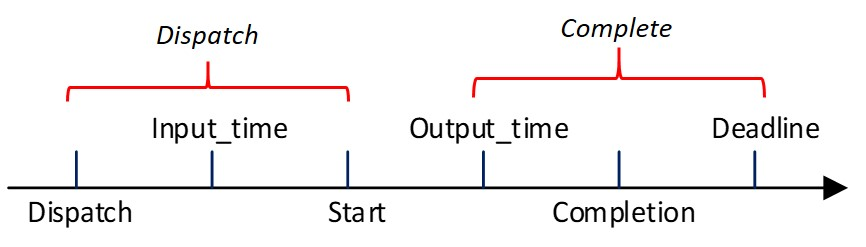
\includegraphics[width=80mm]{aadl_events.jpg}
%\caption{An AADL Model with AGREE Contracts\label{motivation}}
%\end{figure}

%In asynchronous AGREE, the \emph{Execution\_Time} property is modelled by the time interval between the \emph{Dispatch} event and the \emph{Complete} event.
%The assumptions hold at the \emph{Dispatch} event \[Dispatch => Assumption\] , and the guarantees hold at the \emph{Complete} event, i.e. \[Complete => Guarantee\] 
%
%% Assumptions
%We make the following assumptions. The \emph{Input\_Time} property value is unspecified, thus default to dispatch time. The \emph{Output\_Time} property value is unspecified, thus default to the execution completion time. The \emph{Queue\_Size} property value is unspecified, thus default to size one. The \emph{Execution\_Time} property represent a single value, not a real range. The \emph{Dispatch\_Protocol} property value is periodic. The \emph{Timing} property value of each connection is unspecified, thus default to immediate connection. There is no simultaneous read and write access to a queue or buffer (data port). If an event data queue or a data port buffer is empty, the most recent data is used. The \emph{Dequeue} occurs at every dispatch. There is no preemption. There is no propagation delay.
%
%% Modelling
%For an output event data port of a thread, the event and data holds till the thread's next \emph{Complete} event. This is represented by the following AGREE contracts.
%
%\begin{math} 
%not Complete => (event(Port) = prev(event(Port), false))
%\end{math} 
%
%\begin{math}
%not Complete => (true -> (Port = pre(Port)))
%\end{math}  
%
%% Rational
%The output event hold models the latching behavior of an event queue (size one). At the end of execution of a thread, an output event may or may not be raised. However, the AGREE contracts representing the functional requirements only ensures an event is raised only at that exact time instant (i.e. \emph{Complete}). The event is latched so that the target thread, once dispatched, samples the correct result. The consideration for the output data hold is similar.
% 
%% Schedule
%In asynchronous AGREE, a schedule defines the sequential execution order of threads. It is specified by the user. It often come from the actual software execution schedule on the target platform (e.g. seL4 domain schedule). Currently AADL does not define a standard format to specify a schedule. We used AGREE \emph{assumption} on each thread's \emph{Dispatch} and \emph{Complete} event to represent a schedule. For example, \emph{assume "schedule" :			ThreadA\_Dispatch = (Frame = 60) and ThreadA\_Complete = (Frame = 70) and ...}